
\documentclass[conference]{IEEEtran}
\usepackage{graphicx}
\usepackage{amsmath}
\usepackage{booktabs}
\usepackage{url}
\usepackage{cite}

\title{SIDA-Guard: A No-Training Quality-Aware Reliability Layer for Deepfake Detection}

\author{\IEEEauthorblockN{Team Name / Author Names}
\IEEEauthorblockA{Department / University\\
Email: your.email@example.com}}

\begin{document}
\maketitle

\begin{abstract}
Deepfake detection has become an important research topic due to the increasing realism of manipulated videos. Existing deepfake detectors usually output a binary prediction, such as real or fake. However, real-world videos are often degraded by lighting flicker, motion blur, ghosting, background noise, or camera instability. These natural visual degradations may reduce the reliability of detector predictions, especially when detectors are applied outside clean benchmark settings. This project proposes SIDA-Guard, a no-training quality-aware reliability layer for deepfake detection. Instead of training a new detector, SIDA-Guard analyzes video quality and estimates whether a detector prediction may be unreliable. The framework generates controlled perturbations on whole-frame, face-region, and background-region areas, records perturbation metadata, extracts whole-frame and fixed face ROI quality metrics, and converts these metrics into an interpretable quality risk score. Experimental results show that whole-frame metrics capture global degradation such as flicker and blur, while fixed face ROI metrics distinguish face-region degradation from background-only degradation. The final risk score assigns the highest risk to mixed whole-frame degradation and the lowest risk to clean videos, demonstrating its ability to provide interpretable reliability warnings for deepfake detection pipelines.
\end{abstract}

\begin{IEEEkeywords}
Deepfake detection, video quality, reliability estimation, face ROI, visual degradation, perturbation analysis
\end{IEEEkeywords}

\section{Introduction}
Deepfake videos are synthetic or manipulated videos in which a person's face or identity is altered using artificial intelligence techniques. As generative models become more powerful, manipulated videos are increasingly difficult to distinguish from real videos. This creates risks for misinformation, digital trust, identity misuse, and online media verification. Because of these risks, deepfake detection has become an important task in computer vision and multimedia forensics.

Most existing deepfake detection systems focus on classification accuracy. Given an input image or video, the detector predicts whether it is real or fake. However, this prediction alone is not always sufficient in real-world scenarios. A detector may perform well on clean benchmark datasets but behave unreliably when the input video contains poor visual quality. For example, videos recorded in real environments may include lighting flicker, motion blur, ghosting, unstable camera motion, compression artifacts, or background noise. These degradations are not necessarily caused by manipulation, but they may affect the detector's decision.

This motivates an important question: the problem is not only whether a video is fake, but also whether the detector's prediction can be trusted. If a real video is low quality and is incorrectly classified as fake, the result may create a false alarm. In practical applications, such false alarms can be harmful because they may lead to wrong accusations or unreliable content moderation decisions.

In this project, we propose SIDA-Guard, a no-training quality-aware reliability layer for deepfake detection. Instead of building or training a new deepfake detector, SIDA-Guard analyzes whether the input video contains visual quality problems that may reduce prediction reliability. The system does not replace existing detectors. Rather, it provides a reliability warning before the detector output is accepted.

The contributions of this project are summarized as follows:
\begin{itemize}
    \item We propose SIDA-Guard, a no-training reliability layer for deepfake detection.
    \item We design controlled perturbations for whole-frame, face-only, and background-only degradation.
    \item We combine whole-frame quality metrics with fixed face ROI quality analysis.
    \item We convert visual quality metrics into an interpretable risk score and warning decision.
\end{itemize}

\section{Related Work}
\subsection{Deepfake Detection Datasets}
Deepfake detection research has been strongly driven by benchmark datasets. FaceForensics++ is one of the early large-scale datasets for face manipulation detection and has been widely used for evaluating deepfake detection methods \cite{rossler2019faceforensics}. The DeepFake Detection Challenge dataset was introduced to support large-scale research on face-swap video detection and includes more diverse subjects and recording conditions \cite{dolhansky2020dfdc}. Celeb-DF is another widely used dataset designed to provide high-quality and more challenging deepfake videos \cite{li2019celebdf}.

\subsection{Deepfake Detection Methods and Benchmarks}
Many deepfake detection methods use convolutional neural networks to classify facial images or video frames. Xception-based detectors have been widely used as strong baselines for manipulated facial image detection \cite{chollet2017xception}. Benchmarks such as DeepfakeBench aim to standardize evaluation protocols for deepfake detection \cite{yan2023deepfakebench}. Although many detectors improve classification accuracy, they usually assume that the input video is suitable for prediction.

\subsection{Robustness and Visual Degradation}
Real-world videos often contain natural degradations such as motion blur, lighting variation, compression, and camera instability. These degradations may not be malicious, but they can affect visual features used by deepfake detectors. Instead of treating all degraded videos as normal inputs, SIDA-Guard explicitly analyzes the quality risk of the input.

\section{Proposed Approach}
\subsection{Overview}
SIDA-Guard is designed as a no-training reliability layer for deepfake detection. The system takes videos as input and analyzes whether visual quality degradation may make detector predictions unreliable. The full pipeline consists of five stages: video sampling, controlled perturbation generation, perturbation metadata recording, quality metric extraction, and quality risk scoring.

\begin{figure}[t]
\centering
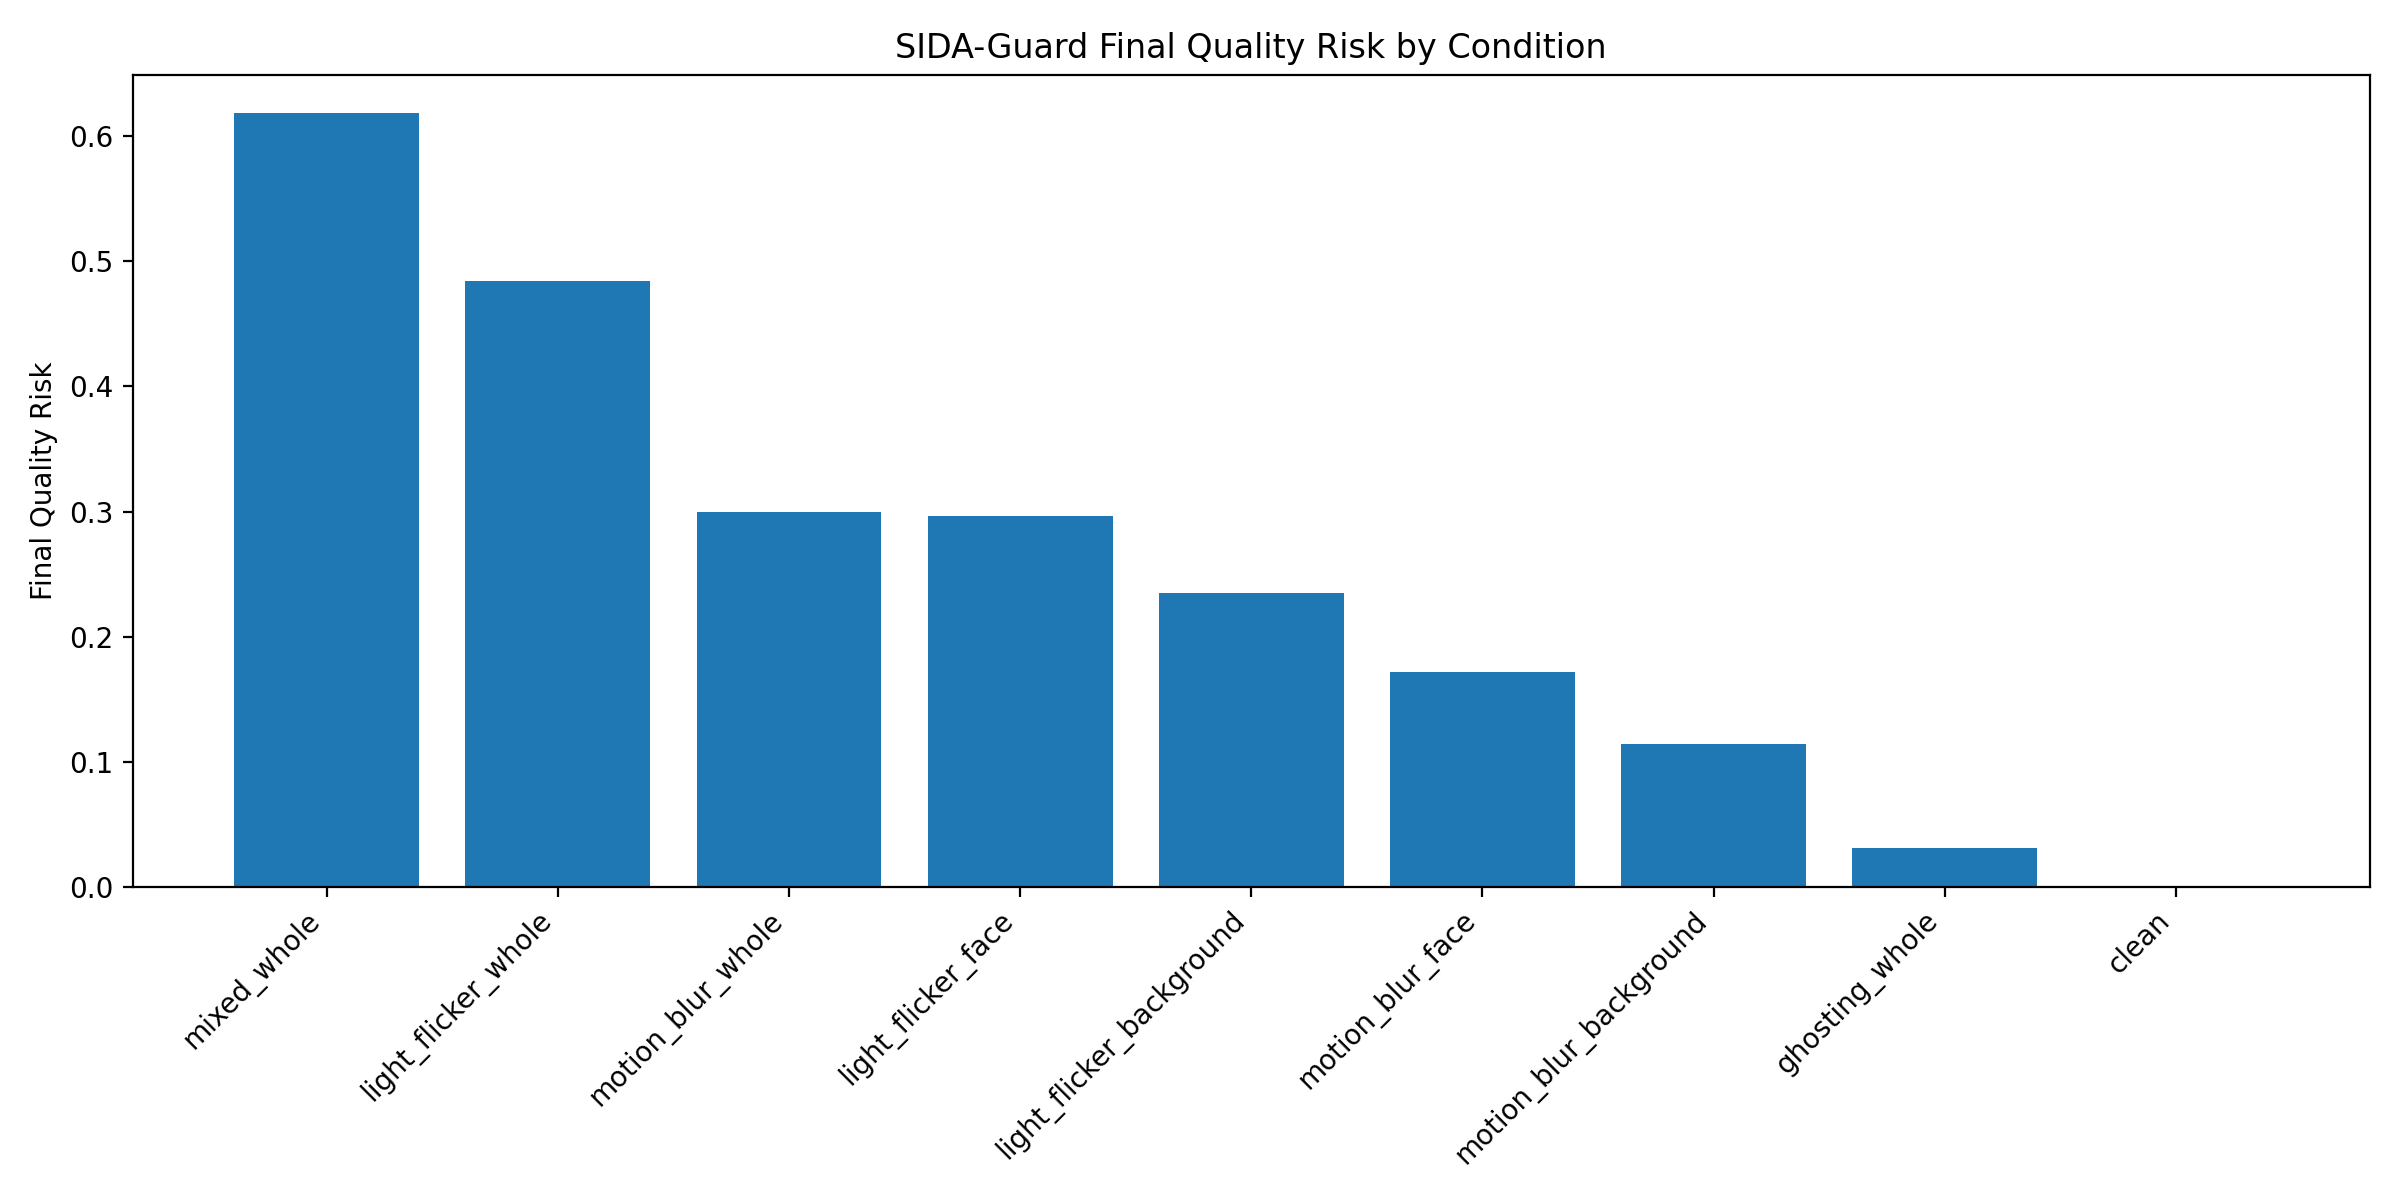
\includegraphics[width=0.95\linewidth]{figures/sida_guard_quality_risk_by_condition.png}
\caption{Example output of SIDA-Guard final quality risk by condition. Replace this with the final figure if needed.}
\label{fig:risk}
\end{figure}

\subsection{Controlled Perturbation Design}
To analyze visual quality risk, we generate controlled perturbations in three regions: whole-frame degradation, face-only degradation, and background-only degradation. Whole-frame degradation modifies the entire video frame. Face-only degradation modifies only the facial region. Background-only degradation modifies the background while preserving the face region. The mixed whole-frame condition combines flicker, motion blur, and ghosting.

\subsection{Perturbation Metadata}
For each generated video, SIDA-Guard records metadata including perturbation type, affected region, start frame, end frame, affected frames, modified frames, and ROI difference score. This metadata ensures that each perturbation is traceable and experimentally controlled.

\subsection{Whole-frame Quality Metrics}
Whole-frame metrics analyze the entire frame. We extract brightness statistics, flicker score, blur score, saturation ratio, and temporal instability. Flicker score is computed based on brightness variation over time. Blur score is computed using image sharpness, where lower values indicate stronger blur. Temporal instability measures frame-to-frame variation.

\subsection{Fixed Face ROI Quality Metrics}
Whole-frame metrics may hide local facial degradation because the face region may occupy only a small part of the frame. To address this issue, SIDA-Guard uses fixed face ROI analysis. The system first detects the face box from the clean video. Then, the same face box is applied to all perturbed versions of the same video. This ensures that the exact same facial area is compared across conditions.

\subsection{SIDA-Guard Risk Score}
SIDA-Guard computes two major risk components: global quality risk and face quality risk. Global risk is computed from whole-frame metrics, while face risk is computed from fixed face ROI metrics. The final quality risk is computed by combining these two components. The reliability score is defined as:
\begin{equation}
R = 1 - Q,
\end{equation}
where $R$ is the reliability score and $Q$ is the final quality risk.

\section{Experimental Analysis}
\subsection{Experimental Setup}
The experiment uses sampled real and fake videos. Each video is processed into multiple conditions, including clean, light flicker, motion blur, ghosting, mixed whole-frame degradation, face-only flicker, face-only blur, background flicker, and background blur.

\subsection{Visual Verification}
Preview images are generated in the form of Original, Perturbed, and Difference. These visual comparisons verify whether the intended region was modified. In face-only perturbations, the difference map should mainly appear around the face. In background-only perturbations, the face region should remain mostly unchanged.

\subsection{Whole-frame Metric Results}
Whole-frame flicker score increases under lighting flicker conditions, especially when the entire frame or background is affected. Whole-frame sharpness score decreases under motion blur conditions. These results show that whole-frame metrics are effective for identifying global degradation.

\subsection{Fixed Face ROI Results}
Fixed face ROI metrics provide more detailed analysis of facial degradation. When the face or the whole frame is affected by flicker, the fixed face flicker score increases. However, when only the background is affected by flicker, the face flicker score remains close to the clean condition. Similarly, when the face or the whole frame is blurred, the fixed face sharpness score decreases, while background-only blur keeps the face sharpness close to clean.

\subsection{SIDA-Guard Risk Score Results}
The final SIDA-Guard risk score assigns the highest risk to mixed whole-frame degradation. In the experiment, mixed\_whole obtains a quality risk score of 0.618 and a reliability score of 0.382. The clean condition receives the lowest risk score of 0.000 and the highest reliability score of 1.000. These results indicate that SIDA-Guard can convert video quality degradation into an interpretable reliability score.

\section{Conclusion}
In this project, we proposed SIDA-Guard, a no-training quality-aware reliability layer for deepfake detection. Instead of training a new detector, SIDA-Guard analyzes whether input video quality may make detector predictions unreliable. The framework generates controlled perturbations, records metadata, extracts whole-frame and fixed face ROI quality metrics, and computes a final quality risk score.

Future work will integrate SIDA-Guard with formal video deepfake detectors such as Xception from DeepfakeBench, evaluate false positive reduction, replace the face detector with a stronger model, and scale the experiment to larger datasets.

\section*{Data Availability Statement}
The source code, README, installation instructions, and dataset information are available in the project GitHub repository. GitHub repository link: \textbf{TO BE ADDED}. Raw video datasets are not included in the repository due to size and dataset access restrictions.

\section*{Code Availability}
All source code used for video sampling, perturbation generation, quality metric extraction, fixed face ROI analysis, and SIDA-Guard risk scoring is included in the GitHub repository under the \texttt{src/} folder.

\bibliographystyle{IEEEtran}
\bibliography{references}

\end{document}
